\section{Fast Fourier Transform}
Fractal terrain generation with a Discrete Fourier Transform has been experimented previously\cite{koh1992fast}.
The idea is to do the inverse transform of pink noise to generate a terrain.
This can be done very quickly with a {\em Fast Fourier Transform} (which will be later referred as FFT). In order to do so, in our parallel implementation we use the {\em FFTW}\cite{fftw} library.
\subsection{Algorithm}
In the first step each process initially generates it's share of complex coefficients with a pink noise damping. This means that in frequency space we have
\be
    P(x_i,y_j) = \frac{z}{(x_i^2+y_j^2)^{\alpha}}
\ee
where $0<\alpha<2$ is a parameter that will determine the roughness of the terrain, and $z$ is a random complex number with a normal distribution.
Since C {\tt stdlib.h} library generates uniformly distributed floating point numbers, this is done with a Box-Muller tranform. 
This is done by taking two independent random variables with a uniform distribution in the range $(0,1)$, say $u_1$ and $u_2$. Then we can generate a complex number $z$ with a normal distribution as following
\be
    z = \sqrt{-2 \ln{u_1}} \exp(2\pi i u_2)
\ee
Since the full height map will be a $L_x L_y$ matrix, each process with have a slice of $L_x L_y / N$ points, where $N$ is the total number of processes used. 

The second step of the algorithm is to perform a parallel FFT  of the points we generated in frequency space. 
In theory we should do an inverse fourier transform, but we can do a direct transform, but this does not change the result qualitatively. 
It also saves some computations as it saves us from a rescaling factor.
The transform is handled by the FFTW library, that has an MPI implementation.
The advantage of this configuration is that the matrix is distributed along the processes, so that the algorithm can handle arrays that are too big to fit on a single process.
The disadvantage of performing an FFT on a distributed memory system is that the algorithm requires to do a transpose, which involves a {\em complete exchange}: each process must communicate to all the others.

Finally, each process writes in order their results to {\tt stdout}; in a tipical usage the user will redirect this output to a file or to {\tt /dev/null} for benchmarking.

One property of this algorithm is that, because of the periodicity of the Fourier transform, it can tiled. As can seen in fig.~\ref{fig:fft3d} the algorithm generates more  ``rolling hills'', due to the smoothness and continuity of the $\sin$ or $\cos$ functions.
\begin{figure}[htb]
\centering
    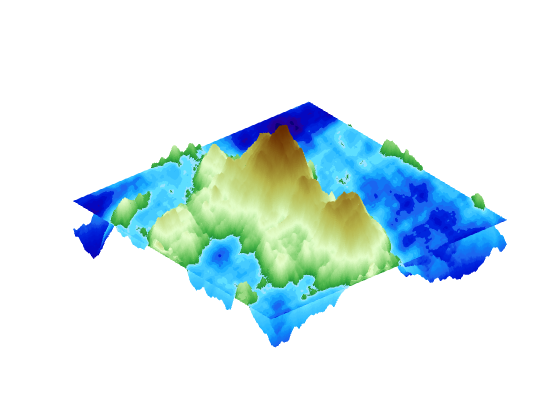
\includegraphics[width=0.8\textwidth]{img/fft3d.png}
    \caption{\label{fig:fft3d}Example of terrain generated with the FFT algorithm ($\alpha=1.1$)}
\end{figure}

\subsection{Performance analysis}
\subsubsection{Complexity}
As before we will estimate the complexity with  a square height map ($L = L_x =  L_y$) with $N$ processes. Since we do not know exactly the complexity of the FFTW routine, but we can estimate that at worst it runs in times comparable to a 2D Cooley-Tuckey algorithm. Therefore, ignoring writing times we have 
\be
    \underbrace{\order(L^2/N)}_{\text{init. of coeffients}} + \underbrace{\order((L \log L)^2/N)}_{FFT} = \underbrace{\order(L^2 \log^2 L/N)}_{\text{overall}}
\ee
\subsubsection{Experimental results}
The benchmarking from parallel runs on the {\em Ferlin} machine using a  number of processes that are powers of 2, for which the FFT is most performant. 
The results are presented in fig.~\ref{fig:benchmarks_time_fft}  and fig.~\ref{fig:benchmarks_speedup_fft}, where we can observe the execution times and the speedup for different height map size and different number of processes. 
We remark that the execution times are quite slower compared to the Diamond-Square algorithm, but this algorithm performs impressively well when the scale becomes larger, since the efficiency $\eta$ is close to 1 (see fig.~\ref{fig:benchmarks_speedup_fft}). The data is presented in table~\ref{table:speedup_fft}.


\begin{table}[H]
\begin{center}
\begin{tabular}{c|c|c|c|c|}
$L$ =  & 3584 & 7168 & 14336 &  \\
\hline
Processes & \multicolumn{3}{c|}{$T_p$ [s]} & {$\bar{S_p}$} \\
\hline
$2$ & 2.266 & 14.683 & 62.276 & 1.80\\
$4$ & 1.190 & 7.700  & 32.173 & 3.44\\
$8$ & 0.676 & 4.250  & 17.863 & 6.17\\
$16$ & 0.406 & 1.973 & 9.206 & 11.9\\
$32$ & 0.236 & 0.843 & 5.060 & 23.7\\
$64$ & 0.116 & 0.436 & 2.180 & 49.3\\

\hline
\end{tabular}
\caption{\label{table:speedup_fft} Running time $T_p$ and average speedup $\bar{S_p}$ for different amount of processes and sizes.}
\end{center}
\end{table}

\begin{figure}[!htb]
\minipage{0.5\textwidth}
    \centering
    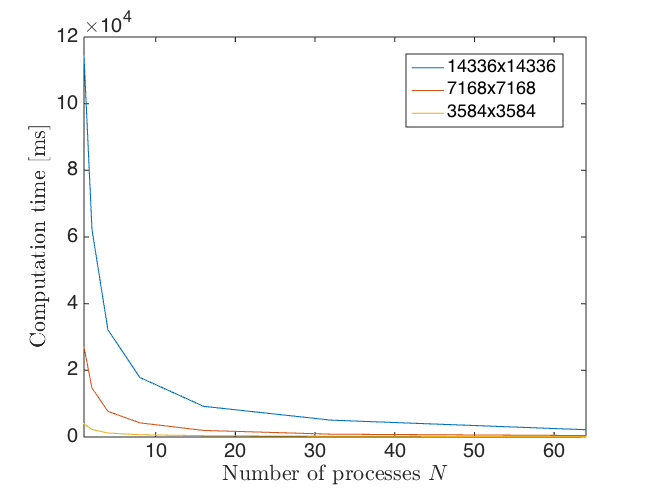
\includegraphics[width=\linewidth]{img/fft_benchmarks1.png}
    \caption{Execution time for the FFT algorithm}
    \label{fig:benchmarks_time_fft}
\endminipage\hfill
\minipage{0.5\textwidth}
    \centering
    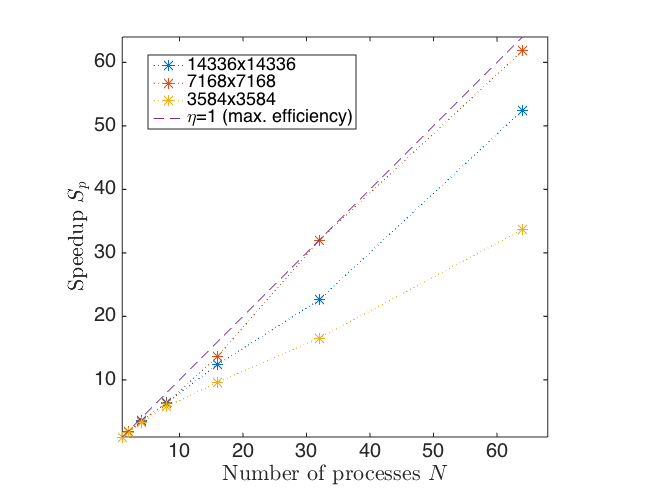
\includegraphics[width=\linewidth]{img/fft_benchmarks2.png}
    \caption{Speedup for the FFT algorithm}
    \label{fig:benchmarks_speedup_fft}
\endminipage\hfill
\end{figure}


